\chapter{Risultati e sviluppi futuri}\label{chapter:Risultati_e_sviluppi_futuri}
%
%
\section{Risultati}\label{sec:cap_sec_subsec}
%
%* TODO: ADD INFO
%TODO: fixhere
Il risultato della web application .NET così sviluppata ha permesso di ottenere numerosi vantaggi, già ampiamente elencati e discussi
nei capitoli precedenti.
\\ \\
Innanzitutto rispetto alla versione originale gestita attraverso un foglio Excel condiviso fra il personale HR e i dipendenti incaricati
di seguire il processo di OnBoarding è stato possibile ottenere una suddivisione di permessi interni al servizio attraverso l'aggiunta di specifici
ruoli con associati specifici permessi, suddividendo così i campi di azione.
La web application inoltre rispetto al sistema iniziale permette di poter gestire più corsi contemporaneamente all'interno della stessa struttura
in maniera più semplice e modulare.
%
\section{Sviluppi fututi}\label{sec:cap_sec_subsec}
\subsection{Pagina statistiche}\label{sec:cap_sec_subsec}
La pagina delle statistiche deve subire un notevole potenziamento, mirando a offrire un'esperienza più completa ed esaustiva.\ 
Questo miglioramento deve concentrarsi sulla possibilità di confrontare una quantità più ampia di dati, 
garantendo al contempo un maggiore spazio dedicato all'analisi dei dati.\ 
Questa evoluzione si rivolge in particolare al personale del reparto HR dell'azienda, 
che ha la responsabilità di gestire il processo di OnBoarding per una varietà di utenti.
\\ \\
Grazie alla capacità di consentire un confronto più dettagliato dei dati, questa pagina deve diventare uno strumento prezioso per l'HR.\ 
Inoltre, dovrebbe essere possibile implementare un numero maggiore di grafici interattivi, che contribuiranno significativamente 
alla comprensione e all'analisi dei dati.
\\ \\
Questo potenziamento non solo agevolerà il processo decisionale dell'HR, ma permetterà anche di individuare con precisione le aree 
che richiedono interventi e miglioramenti.\ In definitiva, mira a trasformare la pagina delle statistiche in uno strumento 
fondamentale per l'ottimizzazione dell'OnBoarding all'interno del contesto dell'azienda.
%
\subsection{Ruoli utente}\label{sec:cap_sec_subsec}
Un'ulteriore evoluzione e arricchimento del sistema potrebbe senz'altro consistere nell'espandere 
l'attuale struttura dei ruoli, che attualmente comprende solo due categorie: ``User'' e ``Admin''.\ 
Questa espansione comporterebbe l'aggiunta di ulteriori ruoli, consentendo così una maggiore granularità nei 
permessi di visualizzazione all'interno delle pagine generate.
\\ \\  
L'implementazione di ruoli aggiuntivi potrebbe essere estremamente vantaggiosa, poiché permetterebbe di adattare 
l'accesso alle informazioni in base alle specifiche responsabilità e autorizzazioni di ciascun utente.\ 
In questo modo, si potrebbe garantire un maggiore controllo sull'accesso ai dati sensibili e una gestione 
più efficiente delle risorse aziendali.
\\ \\
Questo approccio fornirebbe ai decision-maker una maggiore flessibilità nella configurazione dei permessi e consentirebbe 
di assegnare ruoli intermedi, ad esempio ``Supervisor'' o ``Manager'', con diritti di accesso mirati alle informazioni rilevanti 
per il loro ruolo.\ Ciò migliorerebbe la sicurezza dei dati e l'efficienza operativa, 
consentendo a ciascun membro del team di accedere solo alle risorse necessarie per svolgere le proprie mansioni.
%
\subsection{Creazione dei Corsi}\label{sec:cap_sec_subsec}
Un aspetto che potrebbe essere considerato di importanza secondaria, ma che indubbiamente contribuirebbe al miglioramento 
significativo dell'esperienza utente, soprattutto dal punto di vista dell'amministratore, 
riguarda la possibilità di creare Corsi o CorsiTemplate in modo più efficiente, attraverso l'utilizzo di un nuovo processo/i di creazione.\ 
Attualmente, questa operazione richiede un processo manuale, ma esistono alternative 
che potrebbero semplificarne notevolmente l'implementazione.
\\ \\
Una di queste opzioni sarebbe consentire agli amministratori di importare direttamente i dati relativi ai Corsi o ai CorsiTemplate 
da fogli Excel.\ Questo approccio eliminerebbe gran parte del lavoro manuale, 
consentendo di caricare rapidamente una quantità significativa di informazioni nel sistema.
\\ \\
Inoltre, potrebbe essere utile considerare l'integrazione di funzionalità native all'interno del sito web per la creazione 
di Corsi o CorsiTemplate.\ Queste funzionalità integrate potrebbero offrire un ambiente più intuitivo e user-friendly 
per la progettazione e la gestione dei Corsi, migliorando ulteriormente l'esperienza dell'amministratore.
\\ \\
In definitiva, anche se questa caratteristica potrebbe essere considerata di importanza secondaria, 
l'implementazione di strumenti per l'importazione da Excel o funzionalità native all'interno del sito 
rappresenterebbe un passo avanti significativo nella semplificazione delle attività legate alla creazione di Corsi e CorsiTemplate, 
contribuendo in modo tangibile all'efficienza operativa complessiva e al miglioramento dell'esperienza dell'utente amministratore. 
\\ \\
\textit{Nota: } attualmente l'unica modalità per la creazione di nuovi Corsi e CorsiTemplate completi di relative Categorie e Step è la seguente:
\begin{enumerate}
    \item creazione del corso;
    \item apertura del corso;
    \item creazione della categoria;
    \item apertura della categoria;
    \item creazione dello step;
\end{enumerate}
%
\subsection{Text editor}\label{sec:cap_sec_subsec}
Attualmente, la feature che consente la scrittura in sintassi Markdown è piuttosto limitata e semplice.\
Potrebbe essere opportuno valutare l'implementazione di un vero e proprio editor di testo dedicato, 
in aggiunta alla possibilità di scrivere il Markdown manualmente.\ Questa aggiunta consentirebbe agli 
utenti di sfruttare gli stili di formattazione e i vantaggi offerti dalla sintassi Markdown in modo molto più facile, 
inclusivo ed intuitivo per tutti.\ Grazie alla presenza di appositi tasti funzione e a un ambiente di scrittura 
appositamente progettato, si potrebbero sfruttare al meglio tutte le potenzialità della formattazione Markdown 
senza la necessità di conoscere a fondo la sua sintassi.\ Questo migliorerebbe notevolmente l'esperienza degli 
utenti e renderebbe l'utilizzo di questa funzionalità ancora più accessibile e versatile.
\\
Di seguito un esempio preso dal programma ``Slack'':
\begin{figure}[ht]
	\centering
	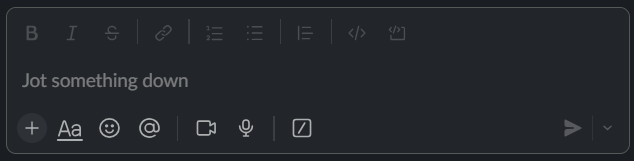
\includegraphics[width=0.7\textwidth]{img/textEditor.png}
	\caption{esempio di un possibile text editor}
	\label{fig:textEditor}
\end{figure}
%
%
\subsection{Reportistica errori e commenti}\label{sec:cap_sec_subsec}
\subsubsection{Reportistica errori}
Una possibile feature futura che potrebbe rivelarsi estremamente utile riguarderebbe 
l'integrazione di un meccanismo avanzato che consenta agli utenti incaricati di svolgere 
i corsi all'interno della piattaforma di segnalare errori o imprecisioni nei task assegnati.\ 
Questa innovativa funzionalità darebbe agli utenti la preziosa possibilità di comunicare direttamente 
agli amministratori eventuali problemi o lacune, come ad esempio link non funzionanti dovuti a modifiche 
nel corso del tempo o informazioni errate nelle assegnazioni.\ Inoltre, potrebbe includere anche la segnalazione 
di descrizioni mancanti o insufficientemente complete, offrendo un quadro completo delle aree da migliorare.
\\ \\
L'introduzione di questa avanzata funzionalità consentirebbe agli amministratori di ricevere feedback costanti 
da parte degli utenti, contribuendo così in modo significativo a elevare la qualità del servizio offerto.\ 
Inoltre, fornirebbe un meccanismo efficace per mantenere sempre aggiornati e corretti i contenuti presenti 
sulla piattaforma, garantendo agli utenti una esperienza di apprendimento completa e senza interruzioni.
\subsubsection{Commenti}
Potrebbe rivelarsi di di grande utilità considerare l'aggiunta di un sistema di assistenza diretta agli utenti 
tramite appositi commenti, in modo che gli utenti possano richiedere aiuto agli amministratori in maniera immediata.\ 
Sistema che potrebbe essere implementato in modo da consentire la comunicazione in threads dedicati, dove 
ogni nuovo messaggio può essere gestito in modo organizzato e pertinente.\ 
Questa funzionalità potrebbe essere integrata insieme alla feature di segnalazione degli errori o essere 
inserita in una sezione separata, per garantire un supporto completo e altamente efficiente per tutti gli utenti finali, 
migliorando notevolmente l'esperienza globale sulla piattaforma.
%
\subsection{Layout della piattaforma}\label{sec:cap_sec_subsec}
Attualmente, il layout della piattaforma si presenta con un design estremamente minimalista, 
concentrandosi esclusivamente su ciò che è strettamente necessario per la corretta visualizzazione 
dei dati e delle informazioni presenti nella piattaforma.\ Questo stile, sebbene efficiente, 
può essere considerato non particolarmente moderno.\ Pertanto, una delle possibili migliorie potrebbe 
consistere nell'apportare alcune modifiche significative al layout stesso, con l'obiettivo di migliorare l'esperienza dell'utente.
\\ \\
Una proposta consisterebbe nell'introduzione di navbar più complete e informative, specialmente per gli amministratori.\ 
Queste navbar potrebbero offrire un accesso rapido alle funzionalità e agli strumenti di amministrazione, 
semplificando così le attività di gestione e supervisione dell'intero sistema.
\\ \\
Inoltre, potrebbe essere benefico considerare l'implementazione di specifiche side-navbar per gli utenti, 
soprattutto quando si trovano nella pagina di visualizzazione dei corsi.\ 
Attualmente, la ricerca di task specifici da completare all'interno di un corso potrebbe risultare disorientante per l'utente finale, 
in quanto potrebbe richiedere uno sforzo eccessivo per individuare le informazioni rilevanti.\ 
L'aggiunta di una side-navbar dedicata potrebbe semplificare notevolmente questa operazione, 
consentendo agli utenti di accedere rapidamente ai alle categorie o ai task all'interno del corso senza difficoltà.
\\ \\
In conclusione, apportare modifiche al layout della piattaforma attraverso l'implementazione di navbar 
più esaustive per gli admin e di side-navbar specifiche per gli utenti, soprattutto nella pagina di visualizzazione dei corsi, 
rappresenterebbe un passo importante per migliorare l'usabilità complessiva del sistema e l'esperienza dell'utente finale.
%
